\section{Estado del arte}

\subsection{Características} %Falta incluir otros modelos que usemos y referencias
Para poder clasificar los audios en reales y generados tenemos que pensar primero en qué datos necesitamos pasarle a los modelos para que aprendan. Podemos separar los datos que debemos pasarle a dichos modelos en 3 grupos.
\begin{enumerate}
	\item Características. Podemos extraer características de la voz como el tono fundamental, los formantes, las pausas, y otros. Con estos datos los modelos pueden aprender las relaciones entre los dos grupos de audios.
	\item Gráficas. Podemos extraer gráficas de la voz como la forma de onda, el espectrograma de MEL, y otros. Con estas gráficas las CNN pueden aprender los puntos clave que diferencian a los audios reales de los generados.
	\item Audio crudo. Existen modelos llamados wav2vec los cuales aprenden directamente de los audios, sacando un vector denso de características latentes en los audios, para después hacer ajuste fino o \emph{fine-tuning} de un modelo para clasificar los audios.  
\end{enumerate}
Con estos 3 enfoques vamos a clasificar los audios y veremos cuál funciona mejor.

\subsection{Modelos de clasificación}
% Poner aquí todo lo referente a modelos IA que hayamos investigado y hayamos usado

\subsubsection{Perceptrón multicapa - MLP}

Un perceptrón multicapa es una red neuronal que se utiliza en aprendizaje supervisado en el campo del aprendizaje automático. El MLP está compuesto por múltiples capas de neuronas interconectadas, en las que las salidas de las neuronas de una capa se convierten en entradas para la siguiente capa. La primera capa se llama capa de entrada, la última capa se llama capa de salida y las capas intermedias se llaman capas ocultas. El MLP presenta una gran capacidad para modelar relaciones no lineales y para generalizar. Como punto negativo del uso de este modelo, podemos remarcar la necesidad de un gran conjunto de datos de entrenamiento para evitar el sobreajuste. Por último, cabe resaltar que los MLP's fueron los precursores de otras redes neuronales más complejas como la redes convolucionales y las redes recurrentes. (Fuente: https://gamco.es/glosario/percepatron-multicapa-mlp/) %Hay que poner la fuente en el .bib

\subsection{Wav2Vec2}
\label{subsubsec:eda_wav2vec}
Wav2Vec2 es un modelo de aprendizaje profundo end-to-end (el modelo procesa todo el flujo de datos, desde la entrada cruda hasta el resultado final) para procesamiento de voz que permite obtener representaciones acústicas de alta calidad directamente desde la señal cruda de audio, sin necesidad de las características del audio~\cite{2020wav2vec}. Fue propuesto por Meta en 2020.

Como parte del entrenamiento, el modelo aprende unidades de habla discreta mediante un gumbel softmax (técnica utilizada en redes neuronales para aproximar el muestreo de distribuciones categóricas discretas de forma diferenciable) para representar las representaciones latentes en la tarea contrastiva.

Tras el preentrenamiento en el habla no etiquetada, el modelo se ajusta con datos etiquetados con una pérdida de Clasificación Temporal Conexionista (CTC\footnote{CTC es un algoritmo y función de pérdida utilizado en redes neuronales profundas para entrenar modelos de aprendizaje automático en tareas de modelado de secuencias cuando los datos de entrada y salida no están alineados.}) para ser utilizada en tareas posteriores de reconocimiento de voz.

El modelo se compone de un codificador de características convolucional multicapa que toma la entrada cruda de audio y devuelve representaciones latentes de voz para T instantes de tiempo. Luego son pasados a un Transformer\footnote{Transformer es un modelo de aprendizaje automático usado en procesamiento de lenguaje natural diseñado para entender y generar secuencias de forma eficiente.} para construir representaciones capturando información de toda la secuencia.

El codificador de características consiste en muchos bloques convolucionales seguidos de una capa de normalización y una función de activación GELU (Gaussian Error Linear Unit). 

GELU pondera las entradas por su probabilidad bajo una distribución gaussiana suavizando su activación cerca de 0.

También realiza representaciones contextualizadas con Transformers donde la salida del codificador se pasa a una red que sigue la arquitectura de un Transformer, y usa una capa convolucional que actua como un embedding posicional relativo.

Por último, Wav2Vec2 consta de un módulo de cuantización que discretiza la salida del codificador a un conjunto finito de representaciones del habla. Esta cuantización se hace con la técnica de Gumbel Softmax.

El entrenamiento del modelo se basa en un preentrenamiento con enmascaramiento en donde se toma la señal de audio y se transforma en representaciones latentes mediante un encoder. Esto se hace por bloques consecutivos de tamaño M que pueden solaparse.

Para cada paso de tiempo enmascarado, el modelo debe identificar la representación latente cuantizada correcta. Para ello, usa una pérdida contrastiva basada en la similitud del coseno.

También se realiza un fine-tuning supervisado para reconocimiento automático del habla usando CTC como función de pérdida y aplicando una versión de SpecAugment (técnica de aumento de datos diseñada específicamente para el reconocimiento automático de voz) para evitar sobreajuste.

\subsection{Random Forest}
\label{subsubsec:eda_rf}

Random Forest es un algoritmo de aprendizaje automático basado en la combinación de múltiples árboles de decisión, propuesto por Leo Breiman en 2001 ~\parencite{2001randomforest}. Pertenece a la familia de métodos \textit{ensemble}, que mejoran el rendimiento agregando las predicciones de varios modelos más simples.

\subsubsection*{Arquitectura y funcionamiento}

El algoritmo construye un ``bosque'' (conjunto) de árboles de decisión donde cada árbol se entrena de forma ligeramente diferente, introduciendo aleatoriedad controlada en dos niveles:

\begin{itemize}
    \item \textbf{Bootstrap aggregating (bagging)}: Cada árbol se entrena con una muestra aleatoria del conjunto de datos original, permitiendo repeticiones.
    
    \item \textbf{Selección aleatoria de características}: En cada división de un nodo del árbol, solo se considera un subconjunto aleatorio de todas las características disponibles.
\end{itemize}

\subsubsection*{Proceso de clasificación}

Cuando llega una nueva muestra de audio con sus características, cada árbol del bosque realiza su propia clasificación. La predicción final se decide por mayoría:

\begin{itemize}
    \item Si la mayoría de los árboles clasifican el audio como deepfake, la predicción final es deepfake.
    \item Si la mayoría lo clasifica como real, la predicción final es real.
\end{itemize}

Este mecanismo de votación reduce drásticamente la varianza del modelo: aunque un árbol individual pueda cometer errores, el consenso del bosque suele ser acertado. Esto se puede ver en la \autoref{fig:voto_mayoria}

\subsubsection*{Hiperparámetros}

Vamos a hablar de los hiperparámetros centrales de Random Forest:

\begin{itemize}
	\item \textbf{n\_estimators}: Define la cantidad de árboles de decisión que conforman el bosque aleatorio. 
	
	\item \textbf{max\_depth}: Controla la profundidad máxima que pueden alcanzar los árboles individuales dentro del bosque.
	
	\item \textbf{min\_samples\_split}: Determina el número mínimo de muestras requeridas para dividir un nodo interno durante la construcción del árbol.
\end{itemize}

\subsubsection*{Ventajas específicas para detección de deepfakes}

Veamos cuáles son algunas de las ventajas de los Random Forest para detección de $deepfakes$:

\begin{itemize}
    \item \textbf{Robustez ante ruido}: Las características de audio pueden contener variaciones por condiciones de grabación; Random Forest maneja bien estos datos ruidosos.
    
    \item \textbf{No requiere normalización}: A diferencia de Redes Neuronales o SVM, no es necesario escalar las características, lo que simplifica el pipeline.
    
    \item \textbf{Resistencia al sobreajuste}: La combinación de $bagging$ y aleatoriedad evita que el modelo memorice el conjunto de entrenamiento.
\end{itemize}

\begin{figure}
	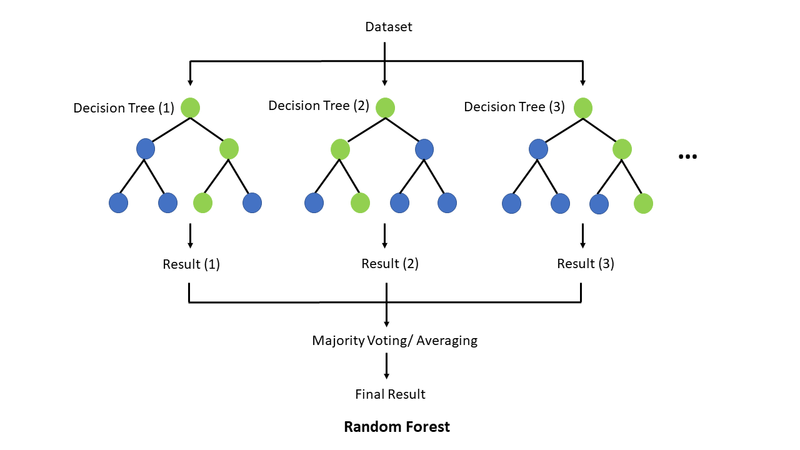
\includegraphics[width=\textwidth]{imagenes/random_forest_majority_vote.png}
	\caption{Voto por mayoría en el ``bosque''.}
	\label{fig:voto_mayoria}
\end{figure}

\subsection{LightGBM}
\label{subsubsec:eda_lgbm}

LightGBM (\textit{Light Gradient Boosting Machine}) es un framework de gradient boosting desarrollado por Microsoft en 2017 ~\parencite{2017lightgbm}. Este modelo optimiza el proceso de entrenamiento mediante innovaciones en la forma de construir los árboles y muestrear los datos. Mientras que Random Forest construye árboles de forma independiente y paralela, LightGBM los construye secuencialmente, donde cada nuevo árbol se especializa en corregir los errores de los anteriores.

\subsubsection*{Arquitectura y funcionamiento}

El proceso de $boosting$ funciona de la siguiente manera:

\begin{enumerate}
    \item Se entrena un primer árbol simple que intenta clasificar las instancias según las etiquetas.
    \item Se identifican las que este primer árbol clasificó incorrectamente.
    \item Se entrena un segundo árbol enfocado específicamente en esos casos difíciles.
    \item Se combinan ambos árboles para mejorar la precisión global.
    \item El proceso se repite construyendo decenas o cientos de árboles, cada uno corrigiendo los residuos de los anteriores.
\end{enumerate}

\subsubsection*{Innovaciones clave}

A continuación mostramos algunos aspectos por los cuales este modelo resulta interesante de aplicar al reconocimiento de voz clonada por IA:

\begin{itemize}
    \item \textbf{Crecimiento por hoja (\textit{leaf-wise})}: Los árboles crecen expandiendo la hoja que más puede reducir el error en cada paso, lo que produce árboles más profundos en las regiones problemáticas y más eficientes en las fáciles.
    
    \item \textbf{Muestreo basado en gradientes (\textit{GOSS, Gradient-based One-Side Sampling})}: Durante el entrenamiento, LightGBM identifica qué instancias tienen mayor error y las prioriza. Esto permite entrenar con datasets grandes sin procesar toda la información redundante.
    
    \item \textbf{Agrupación de características (\textit{EFB, Exclusive Feature Bundling})}: LightGBM agrupa las características que no suelen tomar valores iguales a 0 para reducir la dimensionalidad.
\end{itemize}

\subsubsection*{Proceso de clasificación}

Cuando una nueva instancia llega para ser clasificada:

\begin{itemize}
    \item Pasa secuencialmente por todos los árboles construidos.
    \item Cada árbol aporta una corrección o ajuste a la predicción anterior.
    \item La suma ponderada de todas las contribuciones produce la clasificación final (probabilidad de pertenecer a una clase).
\end{itemize}

\subsubsection*{Hiperparámetros}

Vamos a explicar los hiperparámetros más conocidos en los modelos LightGBM: 

\begin{itemize}
	\item \textbf{max depth}: Limita la profundidad máxima que pueden alcanzar los árboles durante el entrenamiento.

	\item \textbf{num leaves}: Determina el número máximo de hojas por árbol.
	
	\item \textbf{learning rate}: También conocido como $shrinkage rate$ o eta \(\eta\), este parámetro controla la velocidad a la que se actualizan los pesos del modelo después de cada iteración de $boosting$.
	
	\item \textbf{n estimators}: Determina el número máximo de iteraciones de $boosting$ que se realizarán, lo que equivale al número de árboles que se construirán.
	
	\item \textbf{reg alpha y reg lambda}: Estos parámetros aplican regularización L1 ($lasso$) y L2 ($ridge$) respectivamente para controlar la complejidad del modelo y prevenir el sobreajuste.
	
	\item \textbf{objective}: Define la tarea de aprendizaje que debe realizar el modelo y la función de pérdida que se optimizará durante el entrenamiento.
	
	\item \textbf{boosting type}: Determina el algoritmo específico que LightGBM utilizará para construir los árboles secuencialmente.
\end{itemize}

\subsubsection*{Ventajas específicas para detección de deepfakes}

Ahora veamos qué ventajas presenta LightGBM para detección de $deepfakes$:

\begin{itemize}
    \item \textbf{Alta precisión}: El enfoque secuencial de corrección de errores suele superar a Random Forest en problemas complejos como la detección de deepfakes.
    
    \item \textbf{Eficiencia computacional}: El muestreo inteligente permite entrenar con grandes volúmenes de audios en menos tiempo que otros métodos de $boosting$.
    
    \item \textbf{Manejo de desequilibrios}: Si existen desbalances entre clases, LightGBM incorpora mecanismos para ponderar las muestras adecuadamente.
    
    \item \textbf{Early stopping}: Se puede configurar para que detenga el entrenamiento cuando añadir más árboles no mejora la validación, evitando sobreajuste.
\end{itemize}

\subsection{Support Vector Machines (SVM)}
\label{subsubsec:eda_svm}

Las Máquinas de Vectores de Soporte (\textit{Support Vector Machines}, SVM) son un conjunto de algoritmos de aprendizaje supervisado desarrollados por Vladimir Vapnik y su equipo en AT\&T Bell Laboratories durante la década de 1990 ~\parencite{1995svm}. Originalmente diseñadas para clasificación binaria, las SVM se han convertido en uno de los métodos más robustos y teóricamente fundamentados del aprendizaje automático.

\subsubsection*{Fundamento y funcionamiento}

El objetivo fundamental de una SVM es encontrar un hiperplano que separe las clases (en nuestro caso dos, voces reales y voces generadas por IA) con el máximo margen posible. La clave de reside en que no cualquier línea divisoria es válida: el algoritmo busca aquella que maximiza la distancia entre la línea y los puntos más cercanos de cada clase. Estos puntos críticos, que ``sostienen'' el margen, reciben el nombre de \textbf{vectores de soporte} (\textit{support vectors}), de donde el algoritmo toma su nombre.

El proceso de entrenamiento de una SVM puede entenderse en los siguientes pasos:

\begin{enumerate}
    \item \textbf{Identificación de vectores de soporte}: El algoritmo examina todos los puntos de entrenamiento (instancias) e identifica aquellas que son más difíciles de clasificar, es decir, las que están más cerca de la frontera entre clases.
    
    \item \textbf{Maximización del margen}: A partir de estos vectores de soporte, la SVM calcula el hiperplano que maximiza la distancia a ambos lados. Este margen máximo proporciona la mejor capacidad de generalización: cuanto más ancho sea el margen, menor será la probabilidad de error al clasificar nuevas instancias.
    
    \item \textbf{Clasificación de nuevas muestras}: Una vez entrenado el modelo, para clasificar una nueva instancia, simplemente se calcula a qué lado del hiperplano se sitúa.
\end{enumerate}

\subsubsection*{El truco del kernel: Separando lo inseparable}

Uno de los mayores desafíos en la clasificación es que las instancias rara vez son linealmente separables en el espacio original de características. Es decir, no existe una línea recta (o hiperplano) que pueda separarlas perfectamente. Para abordar esta limitación, las SVM introducen el concepto de \textit{kernel} o núcleo.

El \textit{truco del kernel} funciona de la siguiente manera conceptual:

\begin{itemize}
    \item Los datos originales (no separables linealmente) se transforman implícitamente a un espacio de mayor dimensionalidad mediante una función matemática.
    \item En este nuevo espacio, es posible que los datos sí sean linealmente separables.
    \item La ventaja del kernel es que realiza esta transformación sin necesidad de calcular explícitamente las coordenadas en el espacio de alta dimensión, lo que sería computacionalmente costoso.
\end{itemize}

Los kernels más comúnmente utilizados son:

\begin{itemize}
    \item \textbf{Kernel lineal}: Asume que los datos son aproximadamente separables por un hiperplano. Útil cuando el número de características es muy grande.
    
    \item \textbf{Kernel polinomial}: Crea fronteras de decisión curvas mediante combinaciones polinómicas de las características originales.
    
    \item \textbf{Kernel RBF (\textit{Radial Basis Function})}: Es el más utilizado en muchos problemas. Proyecta los datos a un espacio de dimensionalidad infinita, permitiendo fronteras de decisión altamente complejas y no lineales. Se basa en la similitud entre muestras medida por distancia euclidiana:

    \[
    K(\mathbf{x}_i, \mathbf{x}_j) = \exp(-\gamma \|\mathbf{x}_i - \mathbf{x}_j\|^2)
    \]

    donde \(\gamma\) controla la influencia de cada muestra: un valor pequeño considera vecindarios amplios (frontera más suave), mientras que un valor grande se enfoca en vecindarios reducidos (frontera más ajustada a los datos).
\end{itemize}

\subsubsection*{Hiperparámetros}

Veamos cuáles son los hiperparámetros más influyentes en los SVM:

\begin{itemize}
    \item \textbf{C}: Controla el equilibrio entre tener un margen amplio y clasificar correctamente los puntos de entrenamiento.
    
    \item \textbf{kernel}: Es la función que transforma los datos a un espacio de mayor dimensión donde puedan ser separables linealmente.
    
    \item \textbf{gamma \(\gamma\)}: Específico de kernels no lineales (RBF, sigmoide o polinomial). Define cuánta influencia tiene un solo punto de entrenamiento.
    
    \item \textbf{probability}: Este parámetro $booleano$ determina si el modelo SVM debe calibrarse para proporcionar estimaciones de probabilidad junto con las predicciones de clase.
\end{itemize}

\subsubsection*{Ventajas específicas para detección de deepfakes}

Repasemos algunas de las ventajas que presentan los SVM para la detección de $deepfakes$:

\begin{itemize}
    \item \textbf{Fundamento teórico sólido}: A diferencia de otros métodos heurísticos, SVM está basada en la teoría de optimización convexa, lo que garantiza que la solución encontrada es óptima (máximo margen global).
    
    \item \textbf{Eficaz en espacios de alta dimensión}: Las características de audio pueden generar vectores de gran dimensionalidad (decenas o cientos de coeficientes). SVM maneja bien esta situación sin colapsar por la maldición de la dimensionalidad.
    
    \item \textbf{Robustez ante overfitting}: La maximización del margen proporciona una regularización natural que mejora la generalización, crucial cuando se trabaja con datasets limitados de voces $deepfake$.
    
    \item \textbf{Versatilidad mediante kernels}: La capacidad de elegir diferentes kernels permite adaptar el modelo a la estructura no lineal de los datos de audio sin necesidad de transformaciones manuales.
\end{itemize}

\subsection{Modelos de explicación}
Los modelos XAI (eXplainable Artificial Inteligence) han cobrado mucha importancia últimamente y más en términos de modelos de clasificación automáticos debido a la necesidad de saber el por qué se clasifican en un sitio u otro cada elemento, en nuestro caso cada audio.

\hspace{.7cm}
Dos modelos muy utilizados son el modelo SHAP (SHapley Additive exPlanations) y el modelo LIME (Local Interpretable Model-agnostic Explanations), que se utilizan para el análisis de audio sintético. SHAP, como ya sabemos, cuantifica la contribución de cada característica a la predicción final y ayuda a visualizar qué bandas de frecuencia son indicativas de manipulación. Viendo que a menudo revela distorsiones en las zonas de alta frecuencia que el detector suele utilizar para clasificar una muestra como "fake". Por otro lado, LIME, crea explicaciones locales perturbando la entrada y observando los cambios en la salida. También vimos que en forense de audio, LIME se utiliza para generar máscaras sobre espectrogramas, señalando los milisegundos específicos donde se detectan inconsistencias fónicas.

\hspace{.7cm}
Además de estos dos modelos, el modelo de Grad-CAM (Gradient-weighted Class Activation Mapping) se usa mucho junto con los modelos basados en CNN, ya que proporciona visualizaciones espaciales de las áreas del espectrograma que activan la decisión del modelo. Esto es importante para identificar si el modelo se está enfocando en anomalías espectrales o en ruido de fondo, por ejemplo.

\hspace{.7cm}
Por tanto, como hemos visto lo más utilizado y útil son técnicas independientes del modelo, como SHAP y LIME, que muestran que características han servido para que el modelo clasifique un audio como "real" o "fake", y complementariamente para modelos específicos de CNN que usan espectrogramas, se usa Grad-CAM, que muestra que zonas del espectrograma influyen más en la decisión del modelo.